\begin{table}[t]
    \centering
    \caption[Noise Warping Algorithm Benchmarking]{Noise warping algorithm benchmarking in terms of Gaussianity, efficiency, and spatial quality and temporal consistency for two image diffusion based applications. $\Uparrow$/$\Downarrow$ indicates a higher/lower value is better.}
    \resizebox{0.9\textwidth}{!}{ % Resize to fit the page width
    \begin{tabular}{l|cc|cccccccc}
        \toprule
        & \multicolumn{2}{c|}{\textbf{Noise w/o warping}} & \multicolumn{8}{c}{\textbf{ Noise warping method}} \\
        & Fixed & Random & Bilinear & Bicubic & Nearest & PYoCo & CaV & HIWYN & InfRes & Ours \\
        \midrule
        & \multicolumn{10}{c}{\textbf{Gaussianity}} \\
        Moran's \textit{I} (index) $\Downarrow$ & -0.00027 & 0.00019 & 0.30 & 0.24 & 0.26 & 0.00023 & -0.00079 & 0.0011 &  0.00036 & 0.00014 \\
        Moran's \textit{I} (p-value) $\Uparrow$ & 0.29 & 0.36 & 0.0 & 0.0 & 0.0 & 0.73 & 0.25 & 0.11 & 0.60 & 0.84 \\
        K-S Test (index) $\Downarrow$ & 0.089 & 0.075 & 0.34 & 0.37 & 0.17 & 0.13 & 0.073 & 0.062 & 0.055 & 0.060  \\
        K-S Test (p-value) $\Uparrow$ & 0.12 & 0.19 & 0.0005 & 0.0004 & 0.04 & 0.08 & 0.27 & 0.42 & 0.50 & 0.44 \\
        \midrule
        & \multicolumn{10}{c}{\textbf{Efficiency at 1024$\times$1024 resolution}} \\
        GPU time (ms) $\Downarrow$
        & $<$ 1 & $<$ 1 & 4.41 & 4.33 & 6.82 & 3.54 & 2.31 & 55.2 & 2.61 & 2.14 \\
        \midrule
                & \multicolumn{10}{c}{\textbf{Super-resolution - DeepFloyd IF}} \\
        LPIPS $\Downarrow$ & 0.29  & 0.29  & 0.60  & 0.62  & 0.55  & 0.28  & 0.28  & 0.29  & 0.28  & 0.29   \\
        SSIM $\Uparrow$ & 0.88  & 0.88  & 0.72  & 0.70  & 0.65  & 0.88  & 0.88  & 0.87  & 0.88  & 0.88  \\
        PSNR $\Uparrow$ & 29.36  & 29.41  & 28.68  & 28.55  & 28.59  & 29.40  & 29.39  & 29.31  & 29.38  & 29.39 \\
        Warping error $\Downarrow$ & 163.84  & 233.65  & 165.90  & 167.95  & 244.72  & 186.63  & 220.28  & 164.35  & 190.82  & 152.04 \\
        \midrule
        & \multicolumn{10}{c}{\textbf{Relighting - DifFRelight}} \\
        LPIPS $\Downarrow$ & 0.33 & 0.31 & 0.40 & 0.41 & 0.73 & 0.35 & 0.35 & 0.36 & 0.35 & 0.33 \\
        SSIM $\Uparrow$ & 0.69 & 0.77 & 0.73 & 0.70 & 0.38 & 0.58 & 0.67 & 0.64 & 0.60 & 0.70 \\
        PSNR $\Uparrow$ & 28.91 & 29.02 & 28.87 & 28.82 & 28.21 & 28.83 & 28.87 & 28.82 & 28.81 & 28.92 \\
        Warping error $\Downarrow$ & 86.65 & 128.11 & 47.53 & 43.57 & 164.42 & 95.24 & 106.77 & 87.72 & 87.97 & 85.82 \\
        \bottomrule
    \end{tabular}
    }
    \label{gwtf_tab:comparisons_image_diffusion}
\end{table}

\section{Experiments}
\label{gwtf_sec:experiments}


\subsection{Gaussianity}

\textbf{Evaluation metrics}. To validate the preservation of spatial i.i.d. Gaussianity, we follow the evaluation protocol outlined by InfRes~\cite{deng2024infinite}. Specifically, we use Moran's \textit{I} to measure the spatial correlation of warped noise and the Kolmogorov-Smirnov (K-S) test to assess normality.

\noindent \textbf{Baselines}. Following HIWYN~\cite{chang2024warped}, we choose the per-frame fixed and independently-sampled noise as oracle baselines for perfect spatial Gaussianity but zero temporal correlation. We choose bilinear, bicubic, and nearest neighbor temporal interpolation as oracle baselines for sufficient temporal correlation but no spatial Gaussianity. We also compare with the recent noise warping algorithms including HIWYN~\cite{chang2024warped} and InfRes~\cite{deng2024infinite}. In line with these papers, we also include baselines \textit{Preserve Your Own Correlation} (PYoCo)~\cite{ge2023preserve} and \textit{Control-A-Video} (CaV)~\cite{chen2023control}, which have perfect Gaussianity but zero and insufficient temporal correlation, respectively.



\noindent  \textbf{Results}. According to \cref{gwtf_tab:comparisons_image_diffusion} 1st section, we observe:

(1) For Moran's I, a value close to 0 indicates no spatial cross-correlation, which is desirable for i.i.d. noise. Our method achieves a Moran's I index of 0.00014 and a high p-value of 0.84, indicating strong evidence for no spatial autocorrelation. Similarly low Moran's I values and high p-values are observed for PYoCo, CaV, HIWYN and InfRes, because they also aim to generate spatially gaussian outputs.

(2) The K-S test compares the empirical distribution of the warped noise to a standard normal distribution. A small K-S statistic and a high p-value indicate the two distributions are similar. Our method obtains a K-S statistic of 0.060 and p-value of 0.44, suggesting the warped noise follows a normal distribution. Comparable results are seen for the other Gaussianity-preserving methods.

(3) In contrast, the bilinear, bicubic, and nearest neighbor warping methods fail to maintain Gaussianity, exhibiting Moran's I values an order of magnitude higher (0.24 to 0.30) with p-values of 0.0, and K-S statistics 3-6 times larger (0.17 to 0.37) with very low p-values ($<$0.05). These results provide strong evidence for the presence of spatial autocorrelation and deviation from normality in the warped noise from these interpolation-based methods.

\subsection{Efficiency}

Noise generation efficiency is measured by wall time profiling on an NVIDIA A100 40GB GPU, generating noise at a resolution of 1024$\times$1024 pixels. We compare with the same baselines as above. According to \cref{gwtf_tab:comparisons_image_diffusion} 2nd section, our method runs faster than the concurrent InfRes and significantly outperforms the most recent published baseline HIWYN by $26\times$, due to our algorithm's linear time complexity. The efficiency is one order of magnitude faster than real time, validating our feasibility to apply noise warping on the fly during video diffusion model fine-tuning.


\subsection{Video editing via image diffusion}

To further validate the effectiveness of our noise warping algorithm, we repurpose off-the-shelf image-to-image diffusion models to perform video-to-video editing tasks in a frame-by-frame manner, without training. Noise is warped using our algorithm and the above baselines based on the RAFT optical flow~\cite{teed2020raft} from input video and fed to two image pre-trained diffusion models: DeepFloyd IF~\cite{stabilityai2023deepfloyd} for super-resolution and DifFRelight~\cite{he2024diffrelight} for portrait relighting. By measuring the quality and temporal consistency of the output video, we can effectively evaluate the spatial Gaussianity and temporal consistency of different noise warping algorithms.

\noindent \textbf{Evaluation metrics}. We use LPIPS~\cite{zhang2018unreasonable}, SSIM~\cite{hore2010image}, and PSNR~\cite{hore2010image} to measure the quality of the output frames w.r.t. ground truth frames. We use warping error~\cite{lai2018learning} to measure temporal consistency (mean square error) between two adjacent generated frames after flow warping.

\subsubsection{DeepFloyd IF video super-resolution}

We evaluate noise warping on DeepFloyd~IF~\cite{stabilityai2023deepfloyd} super-resolution using 43 videos from the DAVIS dataset~\cite{pont20172017}. The videos were downsampled to the 64$\times$64 and super-resolved to 256$\times$256.

\noindent \textbf{Results}. According to \cref{gwtf_tab:comparisons_image_diffusion} 3rd section, our algorithm outperforms all the baselines in terms of temporal consistency (warping error). Our supplementary video also shows that our algorithm is more stable for the foreground, background, and edges, in contrast to InfRes which is often unstable in the background and HIWNY which is much less stable around moving edges. Our algorithm is comparable to other methods in PSNR, SSIM, and LPIPS image quality metrics, apart from the bilinear, bicubic, and nearest methods which result in low quality generation due to spatial non-Gaussianity. See \cref{gwtf_fig:supp_davis_deepfloyd} in the supplementary material for more details.

\subsubsection{DifFRelight video relighting}

We evaluate noise warping on DifFRelight~\cite{he2024diffrelight} portrait video relighting using their own dataset, which includes 4 subjects in 4 scenarios: a 180-degree view animation, a 720-degree view animation, a zigzag camera movement sequence, and an interpolating camera path through several fixed stage capture positions, all with fixed lighting conditions. During inference, we center crop a 1024$\times$1024 region out of a 1080$\times$1920 Gaussian splat rendering and infer with various noises using conditioned lighting.

\noindent \textbf{Results}. According to \cref{gwtf_tab:comparisons_image_diffusion} 4th section, throughout all baseline comparisons, our algorithm shows consistently advantageous scores in both image and temporal metrics, validating its fundamental benefits to the image diffusion model. Although our visual results at first glance are comparable to HIWYN and InfRes in the supplementary \cref{gwtf_fig:supp_diffrelight_noisewarp} and our \href{https://eyeline-research.github.io/Go-with-the-Flow/}{webpage}, its visual improvements can be seen in the beard regions and skin reflections. We also notice quite low warping error values on the bilinear and bicubic noise inferences, likely coming from the long blurry streaks generated along the flow, while at the same time image quality deteriorates significantly.

\begin{figure}
    \centering
    \includegraphics[width=\linewidth]{src/4_GWTF/fig/comparisons_video_diffusion_object_motions_new_compressed.pdf}
    \caption[Local Object Motion Control Comparisons]{Qualitative comparisons of local object motion control. Zoom in for details. The user selects any number of polygons, then scales, rotates, or translates them along arbitrary paths, which are then used to create the warped noise flow.}
    \label{gwtf_fig:comparisons_video_diffusion_object_motions}
\end{figure}

\begin{figure}
    \centering
    \includegraphics[width=\linewidth]{src/4_GWTF/fig/comparisons_video_diffusion_turning_object.png}
    \caption[Camera Movement Comparisons]{Qualitative comparisons of camera movement video generation of our method (b) and MotionClone (c) using a turning source video (a).}
    \label{gwtf_fig:comparisons_video_diffusion_turning_object}
\end{figure}

\subsection{Video diffusion with motion control}

\subsubsection{Local object motion control}

We introduce a novel method for controlling object motion, by leveraging the flows of input templates. These templates include user-defined local region masks and cut-and-drag trajectories that allow users to specify the motion of one or more objects built with a simple, intuitive UI (\cref{gwtf_fig:comparisons_video_diffusion_object_motions}), and synthetic flows of a camera rotating around 3D objects (\cref{gwtf_fig:comparisons_video_diffusion_turning_object}).

During inference, we use the precise flow computed from the input template frames to guide noise warping for video generation. This enables our I2V model to apply accurate, localized movements and adjustments to the input image while preserving object structure and faithfully following the intended motion trajectory.

We also provide quantitative benchmarks. Following \citep{namekata2024sg}, we use the VIPSeg \cite{miao2021vspw} to benchmark our method on local object motion control, as well as the 40 videos from our user study.

\noindent \textbf{Baselines}. We evaluate our video generation model against five state-of-the-art baselines, SG-I2V~\cite{namekata2024sg}, MotionClone~\cite{ling2024motionclone},
DragAnything~\cite{wu2024draganything}, to benchmark its ability to accurately control object and camera movements derived from a given input template. One of the most recent works, SG-I2V, is an I2V model for object motion transfer guided by bounding box trajectories. We adapt our user-defined polygons to bounding boxes as its input.

\noindent \textbf{Results}. From ~\cref{gwtf_fig:comparisons_video_diffusion_object_motions}, \cref{gwtf_fig:comparisons_video_diffusion_turning_object}, \cref{gwtf_tab:comparisons_video_diffusion_motion_transfer} and our \href{https://eyeline-research.github.io/Go-with-the-Flow/}{webpage}, we observe:

(1) Existing methods struggle to handle complex, localized object motions. Specifically, when specifying local adjustments, such as rotating a dog's head while keeping the rest of the body static, these methods often fail, applying unnatural translational or global transformations to the entire object.

(2) We find that SG-I2V frequently misinterprets object-specific movements as global camera shifts, resulting in scene-wide translations rather than accurate object manipulations.

(3) DragAnything, which employs single-line trajectory control, lacks temporal and 3D consistency, leading to significant distortions and reduced fidelity in complex motion scenarios.

(4) MotionClone also fails to capture subtle object dynamics, as it relies on sparse temporal attention for motion guidance and is likely limited by the low spatial resolution of its diffusion features.

(5) Qualitatively, our model outperforms these baselines by maintaining high object fidelity and 3D consistency, even in scenarios with intricate or overlapping motions. Notably, our approach preserves object integrity and introduces plausible physical interactions, such as generating realistic splashes when moving a duck within a tub. Extensive user studies and quantitative evaluations validate our superior performance in motion consistency, visual fidelity, and overall realism.

(6) Our quantitative evaluation matches our qualitative observations. On both VIPSeg and the 40 videos from our user-study, our method outperforms all the training-based and training-free baselines.


\noindent \textbf{User study}. We conducted a comprehensive user study with 40 participants, asking them to evaluate and rate different methods based on their effectiveness in object motion control and maintaining 3D and temporal consistency. Our method stands out significantly, achieving a win percentage of \textbf{82\%} for cut-and-drag local object motion control like~\cref{gwtf_fig:comparisons_video_diffusion_object_motions} and \textbf{90\%} for the turnable camera movement control like~\cref{gwtf_fig:comparisons_video_diffusion_turning_object}. The three baselines have substantially lower performance levels. More user study details are included in the supplementary material \cref{gwtf_sec:supp_user_study} and \cref{gwtf_fig:supp_user_study_screenshots_statistics}.

\begin{figure}
    \centering
    \includegraphics[width=\linewidth]{src/4_GWTF/fig/comparisons_davis_i2v_new_compressed.pdf}
    \caption[Motion Transfer T2V on DAVIS]{Qualitative comparisons of motion transfer T2V on the DAVIS dataset. Zoom-in needed.}
    \label{gwtf_fig:comparisons_davis_i2v}
\end{figure}

\begin{figure}
    \centering
    \includegraphics[width=\linewidth]{src/4_GWTF/fig/wonderjourney_comparison.png}
    \caption[3D Scene Generation via Depth Warping]{We apply our method to a sequence of frames warped using monocular depth estimation, enabling consistent 3D scene generation from a single image. In this example, we use results from WonderJourney. Zoom-in needed.
    }
    \label{gwtf_fig:comparisons_video_diffusion_WonderJourney}
\end{figure}

\begin{figure}
    \centering
    \includegraphics[width=1\linewidth]{src/4_GWTF/fig/depthwarp.jpg}
    \caption[Depth-Based 3D Scene Exploration]{We explore a 3D scene, flying into a given image. Similar to \cref{gwtf_fig:comparisons_video_diffusion_WonderJourney}, we take an image as an input and use a monocular depth estimator DepthPro \cite{bochkovskii2024depthprosharpmonocular} to get a depth map. Then, we use that depth to generate a crudely warped video (note the pixelation on the rough depth warp column when zoomed in) - and from the movement in that video get warped noise. From there, we run our motion-conditioned I2V model.}
    \label{gwtf_fig:depth_warp}
\end{figure}

\begin{figure}
    \centering
    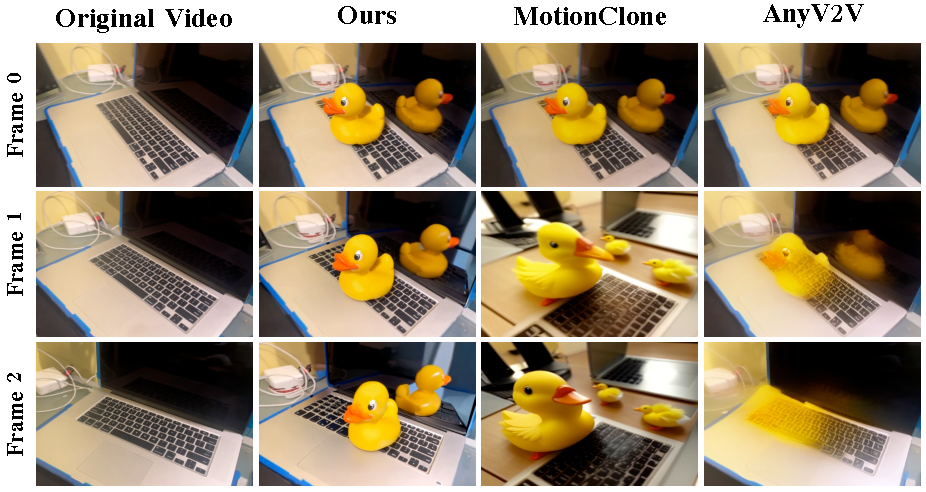
\includegraphics[width=1\linewidth]{src/4_GWTF/fig/InitialFrameAll.pdf}
    \caption[Initial Frame Video Editing Comparison]{Comparison of initial frame video editing results across different methods. All methods start with the same edited initial frame derived from the original video.}
    \label{gwtf_fig:init_frame_edit}
\end{figure}


\subsubsection{Motion transfer and camera movement control}

Our method also supports motion transfer and camera movement control, working with both T2V and I2V video diffusion models. By using reference videos and applying noise warping based on their optical flows, it can effectively capture and transfer complex motions.

\noindent \textbf{Datasets}. We choose the DAVIS video dataset~\cite{pont20172017} containing 43 videos of general object motion with ground truth object segmentation annotations, a random subset of 100 videos from the DL3DV dataset~\cite{ling2024dl3dv}, and 19 videos generated with WonderJourney~\cite{yu2024wonderjourney} that predominantly feature camera movements (\cref{gwtf_fig:comparisons_video_diffusion_WonderJourney}), which itself uses depth-warping.

\noindent \textbf{Evaluation metrics}. For pixel quality, we calculate Fr\'{e}chet Inception Distance (FID) between a set of real and generated frames. For motion controllability, we calculate (1) the mean Interaction over Union (mIoU) of CoTracker's tracking bounding boxes~\cite{karaev2023cotracker} between ground-truth and generated videos, and (2) the pixel MSE between ground-truth and generated videos, considering an I2V diffusion model is conditioned on ground-truth prompts, ground-truth initial frames, and ground-truth motion trajectories/flows. For text controllability, we calculate the cosine similarity between the prompt's CLIP~\cite{radford2021learning} text embedding and the generated frames' CLIP image embeddings, and average over frames of a generated video. For temporal consistency, we calculate (1) the cosine similarity of the CLIP image embeddings between two consecutive generated frames and average over all pairs in a generated video, and (2) the Fr\'{e}chet Video Distance (FVD)~\cite{unterthiner2018towards} between a set of real and generate videos. In addition, we also benchmark on four metrics of VBench~\cite{huang2024vbench}, specifically for the temporal consistency/smoothness dimension.

\begin{table}
    \centering
    \caption[Quantitative Motion Transfer Comparisons]{Quantitative comparisons of motion transfer. $\Uparrow$/$\Downarrow$ indicates a higher/lower value is better. \textbf{Bold} indicates the best results. \colorbox{gray!20}{Gray background rows} indicate our final model. Dashed lines separate ablation study from baseline benchmarking.}
    \definecolor{Gray}{gray}{0.8}
    \resizebox{\linewidth}{!}{
        \begin{tabular}{l|c|ccccccccccc}
        \toprule
        & & & CoTracker & {Optical} & Pixel & CLIP & CLIP & FVD & \multicolumn{4}{c}{VBench $\Uparrow$} \\
        & {Training} & FID & mIoU & {flow} & MSE & text & image & $\times 10^3$ & Subject & Background & Motion & Temperal \\
        & {free?} & $\Downarrow$ & $\Uparrow$ & {err.} $\Downarrow$ & $\Downarrow$ & $\Uparrow$ & $\Uparrow$ & $\Downarrow$ & consistency & consistency & smoothness & flickering\\
        \midrule
        & & \multicolumn{11}{c}{{\textbf{Local object motion control on VIPSeg}}}\\
        MotionClone & \checkmark & 85.2 & 0.71 & 0.48 & 0.086 & 0.31 & 0.95 & 1.26 & 0.88 & 0.85 & 0.94 & 0.90\\
        SG-I2V & \checkmark & 61.4 & 0.63 & 0.84 & 0.065 & 0.31& 0.97 & 1.06 & \textbf{0.93} & \textbf{0.95} & 0.96 & 0.94\\
        \rowcolor{Gray} Ours & $\times$ & \textbf{41.1} & \textbf{0.75} & \textbf{0.36} & \textbf{0.039} & \textbf{0.32} & \textbf{0.98} & \textbf{0.47} & 0.91 & 0.92 & \textbf{0.97} & \textbf{0.95} \\
        \midrule
        & & \multicolumn{11}{c}{{\textbf{Local object motion control on our 40 samples in the user study}}}\\
        MotionClone & \checkmark & 96.6 & - &  0.80 & 0.048 & \textbf{0.33} & \textbf{0.98} & 1.38 & 0.86 & 0.93 & 0.97 & 0.95 \\
        SG-I2V & \checkmark & 79.9 & - &  0.64 & 0.042 & 0.32 & \textbf{0.98} & 1.27 & 0.95 & \textbf{0.95} & \textbf{0.98} & 0.94 \\
        DragAnything & $\times$ & 82.8 & - & 0.62 & 0.047 & 0.31 & 0.97 & 1.30 & 0.93 & \textbf{0.95} & \textbf{0.98} & 0.95 \\
        \rowcolor{Gray} Ours & $\times$ & \textbf{74.3} & - & \textbf{0.56} & \textbf{0.028} & 0.32 & \textbf{0.98} & \textbf{0.94} & \textbf{0.96} & \textbf{0.95} & \textbf{0.98} & \textbf{0.96} \\
        \midrule
        & & \multicolumn{11}{c}{\textbf{Motion transfer T2V on DAVIS}}\\
        DMT & \checkmark & - & \textbf{0.85} & \textbf{0.28} & - & 0.31 & 0.95 & - & 0.86 & 0.92 & 0.94 & \textbf{0.91} \\
        MotionClone & \checkmark & - & 0.75 & 0.38 & - & 0.32 & 0.93 & - & 0.78 & 0.89 & 0.86 & 0.81\\
        {MotionCtrl} & $\times$ & & 0.47 & 0.85 & -& 0.32 & 0.97 & - & 0.97 & 0.93 & \textbf{0.98} & 0.92  \\
        \rowcolor{Gray} Ours & $\times$ & - & 0.70 & 0.41 & - & \textbf{0.33} & \textbf{0.98} & - & 0.88 & \textbf{0.93} & 0.97 & 0.89\\
        \hdashline
        {Ours-CogVideoX-2B} & $\times$ & - & 0.64 & 0.48 & - & 0.32 & 0.95 & - & 0.89 & 0.91 & 0.97 & 0.90\\
        \midrule
        & & \multicolumn{11}{c}{\textbf{Motion transfer I2V on DAVIS}}\\
        MotionClone & \checkmark & 99.4 & 0.72 & 0.42 & 0.068 & 0.31 & 0.94 & 1.84 & 0.75 & 0.85 & 0.92 & 0.87 \\
        {ImageConductor} & $\times$ & 104.6 & 0.66 & 0.64 & 0.072 & 0.31 & 0.93 &  1.58 & 0.77 & 0.88 & 0.93 & 0.90 \\
        Original CogVideoX-5B & \checkmark & \textbf{76.62} & 0.52 & 0.67 & 0.088 & 0.31 & 0.96 & 1.36 & 0.85 & 0.91 & 0.96 & 0.92 \\
        \rowcolor{Gray} Ours ($\gamma=0.5$) & $\times$ & 78.6 & \textbf{0.74} & \textbf{0.36} & \textbf{0.053} & 0.31 & \textbf{0.97} & \textbf{1.21} & \textbf{0.88} & \textbf{0.92} & \textbf{0.98} & \textbf{0.93}\\
        \hdashline
        {Our ($\gamma=0.9$)} & $\times$ & 92.5 & 0.50 & 0.65 & 0.072 & 0.31 & 0.95 &  1.59 & 0.80 & 0.89 & 0.94 & 0.91\\
        {Our ($\gamma=0.8$)} & $\times$ & 80.6 & 0.68 & 0.47 & 0.067 & 0.31 & 0.96 & 1.50 & 0.85 & 0.91 & 0.96 & 0.92 \\
        {Our ($\gamma=0.4$)} & $\times$ & 77.7 & 0.74 & \textbf{0.36} & 0.056 & 0.31 & 0.97 & 1.27 & 0.87 & 0.91 & 0.97 & \textbf{0.93}\\
        {Our ($\gamma=0.2$)} & $\times$ & 77.1 & 0.74 & 0.37 & 0.058 & \textbf{0.32} & 0.97 & 1.29 & 0.86 & 0.91 & 0.97 & \textbf{0.93}\\
        \hdashline
        {Our (33\% data)} & $\times$ & 100.1 & 0.73 & 0.40 & 0.066 & 0.31 & 0.97 & 1.46 & 0.85 & 0.90 & 0.97 & 0.92\\
        {Our (12.5\% data)} & $\times$ & 105.2 & 0.71 & 0.39& 0.072 & 0.31 & 0.96 & 1.93& 0.84 & 0.89 & 0.97 & 0.91\\
        \midrule
        & & \multicolumn{11}{c}{\textbf{Camera movement transfer I2V on DL3DV}}\\
        MotionClone & \checkmark & 82.7 & 0.71 & 0.44 & 0.104 & \textbf{0.33} & 0.94 & 1.11 & 0.74 & 0.85 & 0.91 & 0.86 \\
        {ImageConductor} & $\times$ & 89.2 & 0.61 & 0.78 & 0.068 & 0.31 & 0.95 & 0.91 & 0.85 & 0.90 & 0.95 & \textbf{0.93}\\
        \rowcolor{Gray} Ours & $\times$ & \textbf{48.4} & \textbf{0.83} & \textbf{0.20} & \textbf{0.046} & 0.32 & \textbf{0.97} & \textbf{0.34} & \textbf{0.88} & \textbf{0.92} & \textbf{0.97} & \textbf{0.93}\\
        \midrule
        & & \multicolumn{11}{c}{\textbf{Camera movement transfer I2V on WonderJourney}}\\
        MotionClone & \checkmark & 177.9 & 0.81 & 0.17 & 0.103 & \textbf{0.32} & 0.96 & 1.93 & 0.75 & 0.87 & 0.93 & 0.87 \\
        {ImageConductor} & $\times$ & 166.1 & 0.79 & 0.39 & 0.085 & \textbf{0.32} & 0.94 & 1.63 & 0.79 & 0.88 & 0.93 & 0.90 \\
        \rowcolor{Gray} Ours & $\times$ & \textbf{128.3} & \textbf{0.85} & \textbf{0.15} & \textbf{0.072} & 0.31 & \textbf{0.98} & \textbf{1.55} & \textbf{0.82} & \textbf{0.91} & \textbf{0.98} & \textbf{0.94}\\
        \bottomrule
    \end{tabular}
    }
    \label{gwtf_tab:comparisons_video_diffusion_motion_transfer}
\end{table}

\noindent \textbf{Baselines}. For the motion transfer T2V scenario, we compare with the recent state-of-the-art methods Diffusion Motion Transfer (DMT)~\cite{yatim2024space}, MotionClone~\cite{ling2024motionclone}, and MotionCtrl~\cite{wang2024motionctrl}. For the motion transfer I2V, we compare MotionClone and ImageConductor~\cite{li2024imageconductorprecisioncontrol}) as DMT does not take an image as input.

In addition, we demonstrate video first-frame editing, a challenge where a user starts with an original video and an edited version of its initial frame. The goal is to seamlessly propagate the edits made to the first frame throughout the entire video while preserving the original motion. We qualitatively compare with MotionClone~\cite{ling2024motionclone} and the state-of-the-art video editing method AnyV2V~\cite{ku2024anyv2v} on real videos with photoshopped first frames.

We also source a few images for image-based depth warping, where we take an image, use a monocular depth estimator, DepthPro~\cite{bochkovskii2024depthprosharpmonocular}, to get a depth map, and crudely warp it to simulate a desired camera trajectory.

\noindent \textbf{Results}.
We present both qualitative and quantitative comparisons with baselines in~\cref{gwtf_tab:comparisons_video_diffusion_motion_transfer}, \cref{gwtf_fig:comparisons_davis_i2v}, \cref{gwtf_fig:comparisons_video_diffusion_WonderJourney}, \cref{gwtf_fig:depth_warp}, \cref{gwtf_fig:init_frame_edit}, and our \href{https://eyeline-research.github.io/Go-with-the-Flow/}{webpage}. We observe:

(1) Our superior object motion transfer: On the DAVIS dataset, which includes object motion along with some degree of camera movement, our method demonstrates improved motion fidelity and overall video quality, as measured by Vbench. In particular, in the I2V setting, where both the initial frame and the source video are provided, our method achieves significantly better scores in FID, FVD, and motion metrics, indicating much closer reconstructions of the ground truth videos.

(2) Our superior camera movement control: On the DL3DV and WonderJourney datasets, which involve substantial camera movement, our method notably outperforms MotionClone in both motion fidelity and general video quality. This highlights our method's ability to effectively replicate intricate camera movements while maintaining visual coherence. For our depth-warping example~\cref{gwtf_fig:depth_warp}, our results are far better than simply warping an image from its depth map, resulting in a smooth, realistic camera trajectory. See our \href{https://eyeline-research.github.io/Go-with-the-Flow/}{webpage} for videos.

(3) Our superior video first-frame editing: In~\cref{gwtf_fig:init_frame_edit}, our method seamlessly integrates the added object into the scene while accurately preserving the camera movement from the original video. In contrast, both baselines exhibit significant identity loss: MotionClone generates additional, unintended objects, and in AnyV2V, the foreground object gradually disappears. This demonstrates the superiority of our method in maintaining the original video's motion while faithfully preserving the identity of the object added to the first frame.


\subsubsection{Ablation studies}


In~\cref{gwtf_tab:comparisons_video_diffusion_motion_transfer} for the DAVIS I2V task, we compare our method with a variant that excludes motion conditioning using warped noise (``Original CogVideoX-5B''), relying solely on textual prompts describing the objects. We observe: (1) Better video reconstruction: Our method, which incorporates motion conditioning, achieves superior FID, FVD, and CoTracker mIoU scores, indicating more accurate reconstruction of the source video. This is because textual prompts and the initial frame alone are insufficient to capture a video's future dynamics, whereas incorporating real video-derived motion guidance enables the generation of more realistic sequences. (2) Improved video quality: By utilizing warped noise for motion conditioning, our approach not only maintains but also enhances overall video quality, as measured by Vbench, demonstrating that integrating realistic motion cues improves the plausibility of the generated videos without compromising quality.

Further exploring the effects of degradation, we find that as the degradation values $\gamma$ increase, the motion control becomes tighter - resulting in higher optical flow and CoTracker-mIoU scores, along with a closer per-frame similarity to target videos on the I2V DAVIS task. We find that, in general, $\gamma\approx 0.5$ is a good value for most tasks.

We also perform ablations on dataset size, comparing models trained on different fractions of our dataset: training with a fraction of dataset yields worse performance than our full model.

In addition, we perform an ablation where we use the weaker base model CogVideoX-2B, and find its performance is weaker than our main T2V model, based on CogVideoX-5B.
